%!TEX root = jt-thesis-main.tex

\section{English Abstract}
\begin{onehalfspace}
	
	The english abstract is required for all english theses at TU-Berlin.
\end{onehalfspace}
\clearpage

\section{Deutscher Abstract}
\begin{onehalfspace}
	
	Ein deutscher Abstract wird immer benötigt, für alle Abschlussarbeiten an der TU-Berlin. 
\end{onehalfspace}
\clearpage

\section{Introduction}
\label{sec:Introduction}

In an essay, article, or book, an introduction (also known as a prolegomenon) is a beginning section which states the purpose and goals of the following writing. This is generally followed by the body and conclusion.

The introduction typically describes the scope of the document and gives the brief explanation or summary of the document. It may also explain certain elements that are important to the essay if explanations are not part of the main text. The readers can have an idea about the following text before they actually start reading it.

ln technical writing, the introduction typically includes one or more standard subsections: abstract or summary, preface, acknowledgments, and foreword. Alternatively, the section labeled introduction itself may be a brief section found side-by-side with abstract, foreword, etc. (rather than containing them). In this case the set of sections that come before the body of the book are known as the front matter. When the book is divided into numbered chapters, by convention the introduction and any other front-matter sections are unnumbered and precede chapter 1.

Keeping the concept of the introduction the same, different documents have different styles to introduce the written text. For example, the introduction of a Functional Specification consists of information that the whole document is yet to explain. If a Userguide is written, the introduction is about the product. In a report, the introduction gives a summary about the report contents. (Source: Wikipedia)

\subsection{Motivation}
\label{sec:motivation}

Put some motivation here...

\subsubsection{Scientific Background}
\label{sec:Scientific Background}

\clearpage
\subsection{Contributions}
\label{sec:contributions}

Clearly point out and describe the contributions of this work

The contributions of this thesis go as follows: 
\begin{enumerate}
	\item This thesis is the first to propose...
	\item We are the first to implement...
	\item We provide the basis for...
	\item The results of this thesis...
\end{enumerate}
\clearpage

\subsection{Thesis Outline}

Provide some outline of your thesis.

\para{Section \ref{sec:Background}.}  In section  \ref{sec:Background}, we present ..., including. Furthermore, we provide ... The section concludes with ...

\para{Section X.} Section X provides a survey through related publications. The section is split in two subsections. First, we provide an overview of ... Thereby, we describe ... We conclude with ...

\section{Taxonomy}
\label{sec:Taxonomy}

In this chapter, we present the backgrounds of this thesis. In ... we present ... Add some short introduction to each section.

\subsection{Overview}
\label{sec:Overview}

This is how you can include a figure and refer to it. It is figure \ref{fig:Example}.

\begin{figure}[h!]
	\begin{center}
		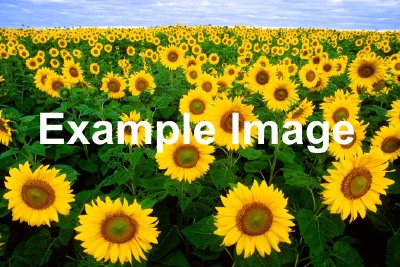
\includegraphics[width=0.5\textwidth]{images/Example.jpg}
		\caption{This is just an example image.}
		\label{fig:Example}
	\end{center}
\end{figure}

%This command prevents images from being floated too far away.
\FloatBarrier

\subsubsection{Adaptive Sampling}
\label{sec:Adaptive Sampling}

This is an example table taken from DIMA's IDB lecture slides:

\begin{table}[h!]
  \begin{tabular}{lccccccc}
	\toprule    
    \hline
    \textbf{Functions} & \multicolumn{3}{c}{\textbf{Framework}} && \multicolumn{2}{c}{\textbf{User Defined}}\\
    \cmidrule{2-4}  \cmidrule{6-7}  
    & Map & Shuffle & Reduce && Mapper &  Reducer\\
    \midrule
    \textbf{Input} & $ (K_m \times V_m)^{*} $ & $ (K_r \times V_r)^{*} $ & $ (K_r \times V_r^{*})^{*} $ && $ (K_m \times V_m) $  & $ (K_r \times V_r^{*}) $\\
    \hline
    \textbf{Output} & $ (K_r \times V_r)^{*} $ & $ (K_r \times V_r^{*})^{*} $ & $ (K_o \times V_o)^{*} $ && $ (K_r \times V_r)^{*} $ & $ (K_o \times V_o)^{*} $\\
	\hline    
    \bottomrule
  \end{tabular}
  \caption{Inputs and outputs of functions and processing phases in Map Reduce.}
  \label{table:mapRedFunctions}
\end{table}

And one more table:

\begin{table}[h!]
  \centering
  \begin{tabular}{lll}
	\toprule    
    \hline
    & \textbf{Input} & \textbf{Output}\\
    \midrule
    File Line 1:& Beer Beer Tea Coffee &\\
    File Line 2:& Tea Tea Beer Tea &\\
	\hline
	Map 1: & (1, Beer Beer Tea Coffee) & [(Beer,1),(Beer,1),(Tea,1),(Coffee,1)]\\
    Map 2: & (2, Tea Tea Beer Tea)     & [(Tea,1),(Tea,1),(Beer,1),(Tea,1)]\\
    \hline
    Reduce 1 & (Beer,[1,1,1])  & (Beer,3)\\  
	Reduce 2 & (Coffee,[1])    & (Coffee,1)\\
	Reduce 3 & (Tea,[1,1,1,1]) & (Tea,4)\\
    \hline    
    \bottomrule
  \end{tabular}
  \caption{Word Count Example: Sample data transformation.}
  \label{table:wcDataTransformation}
\end{table}

\subsubsection{Compressive Sampling}

You may want to use the description environment for your definitions.

Vocabulary introduced by Hirzel et al.~\cite{hirzel2014catalog} and inspired by Gamma et al.~\cite{gamma1995} and Fowler et al.~\cite{fowler1999}.

\begin{description}
	\item[Data Stream] \textit{A conceptual/possibly infinite sequence of data-items which comes from a stream source. Streaming systems implement streams as \ac{FIFO} queues.}
	\item[Stream Source] \textit{A stream source is a data source that possibly emits an infinite number of data-items.}
	\item[Operator] \textit{A code block , which consumes data-items from incoming stream(s) and produces data-items on outgoing stream(s). Thereby it performs a continuous data transformation.}
	\item[Query] \textit{A streaming query consists of operators which are vertices in a graph. The edges of the graph represent the data flow between operators. A streaming query combines multiple operations to a data transformation flow. Queries are also called \textit{applications}.}
	\item[Data-item] \textit{The smallest unit of data, which is processed by the streaming query, is called \emph{data-item}. It is also the smallest unit of communication along edges in the query. Anyhow, data-items can consist of several attributes.}
	\item[Window] \textit{A finite subsequence or chunk of data-items from a stream.}
\end{description}

\subsubsection{Data Sharing}
\label{sec:Listings}

Listing \ref{lst:SPLexample} is an example for a listing using lstlisting.

\begin{lstlisting}[float=b,label=lst:SPLexample,caption={An IBM SPL code example}]
stream<MyType> outputName = Aggregate(InputStream){
	window InputStream : sliding, delta(...), count(...);
	output outputName  : attribute1=Sum(a1*a2), attribute2=Sum(a3);
}
\end{lstlisting}

% Listings can also be imported from files like listing \ref{lst:samplecode}.
% \lstinputlisting[label=lst:samplecode,caption=A Java Hello World Program,language=java]{listings/helloWorld.java}
%Also use: firstline=300,lastline=500, linerange={10-17,20-35}


\subsection{Discussion}
\label{sec:Discussion}

Lorem ipsum dolor sit amet, consectetur adipisici elit, sed eiusmod tempor incidunt ut labore et dolore magna aliqua. Ut enim ad minim veniam, quis nostrud exercitation ullamco laboris nisi ut aliquid ex ea commodi consequat. Quis aute iure reprehenderit in voluptate velit esse cillum dolore eu fugiat nulla pariatur. Excepteur sint obcaecat cupiditat non proident, sunt in culpa qui officia deserunt mollit anim id est laborum.

\subsubsection{Other Algorithms}
\label{sec:Listings}

Lorem ipsum dolor sit amet, consectetur adipisici elit, sed eiusmod tempor incidunt ut labore et dolore magna aliqua. Ut enim ad minim veniam, quis nostrud exercitation ullamco laboris nisi ut aliquid ex ea commodi consequat. Quis aute iure reprehenderit in voluptate velit esse cillum dolore eu fugiat nulla pariatur. Excepteur sint obcaecat cupiditat non proident, sunt in culpa qui officia deserunt mollit anim id est laborum.


\subsubsection{Combination of Algorithms}
\label{sec:Listings}

Lorem ipsum dolor sit amet, consectetur adipisici elit, sed eiusmod tempor incidunt ut labore et dolore magna aliqua. Ut enim ad minim veniam, quis nostrud exercitation ullamco laboris nisi ut aliquid ex ea commodi consequat. Quis aute iure reprehenderit in voluptate velit esse cillum dolore eu fugiat nulla pariatur. Excepteur sint obcaecat cupiditat non proident, sunt in culpa qui officia deserunt mollit anim id est laborum.


\subsection{Acronyms}
\label{sec:Acronyms}

There are many acronyms provided in this template. You can use them as follows:
\begin{itemize}
	\item \acs{CSV} - The acs-command always uses the short form.
	\item \ac{CSV} - The ac-command uses the long form for the first appearance, then the short form.
	\item \acl{CSV} - The acl-command forces to use the long form.
	\item \acp{CSV} - When adding a 'p' to the mentioned commands, the plural form will be used.
\end{itemize}

\subsection{Citations}
You should read the publications from Albert Einstein~\cite{einstein1920relativity}.

\section{Conclusion}
\label{sec:Conclusion}

It is very important to have a good conclusion.